\chapter{Diffusion and discussion of results}

This chapter aims to summarize the results of this thesis and to critically discuss them.
Furthermore, the results should be set into perspective with literature to better emphasize the potential
and make the reuslts comparable. 
Wherever possible a generalization of results should be established.

\section{Solution architecture and Hyperparameter tuning}

The first result is the developed \ac{IT}-artifact\ref{Overall architecture} as overall solution architecture. 
The required components for the combination of the digital computer with the \ac{mem-HNN} accelerator 
is universally valid and can be used to train Boltzmann Machines with the Hopfield Neural Network as sampling method. 
This is validated by the successful \ac{DSR} outcomes that proved the possibility of efficiently 
training a Boltzmann Machine with a good prediction accuracy.
Despite, the training is done by a simulation and not done on the actual \ac{mem-HNN}, which can be seeen as critics 
all the calculations and hardware components are correctly mapped in the software and are validated by each iterative design and evaluation phase.
Furthermore, this procedure is part of the \ac{ASIC} design process before building and using the physical accelerator.


In the next step, the baselines for training are established using Gibbs sampling and the Metropolis Hastings algorithm.
\textbf{Gibbs Sampling} is the most \textbf{sensitive} method and has a prediction accuracy of \(\mathbf{92.29\%}\), while
\textbf{Metropolis Hastings} is far more stable with a faster learning curve and an total prediction accuracy of \(\mathbf{94.15\%}\).
With the created Baselines, the implementation of the noisy injected Hopfield Network is achieved, which is considered the main result for the thesis. 
Continuation of known proof of concepts, a full training for the noise injected Hopfield Network is done by adding a random gaussian distribution 
to the activation function of the \ac{RBM} shown in \ref{Noisy_acitivation_function_good}. 
First, the metric predition accuracy is of interest, since this helps to compare the performance with the other two conventional sampling methods.

Hence, the \textbf{asynchronously Hopfield Network} achieved an baseline of \(\mathbf{90.81\%}\) without Hyperparameter tuning but has a more stable  learning rate than Gibbs Sampling and
is equal with Metropolis Hastings.
Here, the Hyperparameter tuning can be highlighted due to the fact that until now there was no data available for such an \ac{IT}-artifact and especially not for the Hopfield Network sampling method.
With some adjustments made to the scale, which represents the standard deviation of the injected noise the stability, the performance is meassured.
The outcome is at a scale of 1.6 the prediction accuracy is the highest of all with a value of \(\mathbf{94.77\%}\) shown in \ref{Hyperparamers_Scale_ohne}.
In comparison, the \textbf{N/2 Half Hopfield Network} has a scale that is \textbf{more sensitive} than the asynchronously approach \ref{Hyperparamers_Scale_mit}.
On the other Hand, its predition accuracy of \(\mathbf{94.76\%}\) is equal since it is an statistical procedure and 0.001 is no significant difference.
In contrast, noticable differences can be seen when looking at the second Hyperparamer ``sampling iterations''. 
Here, the \textbf{asynchronously Hopfield Network} approach requires at least \textbf{4000 iterations} to achieve good results topping out with
a prediction accuracy of \(\mathbf{94.5\%}\) at 15000 sampling iterations. 
Meanwhile, the \textbf{N/2 Half Hopfield Network} updats about 25\% of all neurons in the network per sampling iteration and 
this results in good achievable prediction accuracys already after \textbf{221 sampling iterations}.
Hence, the best prediction accuracy with \(\mathbf{95.1\%}\) is the best out of all approaches with the least sampling iterations \ref{Hyperparamers_Iteraions_mit}.
Compared to the asynchronous update it is about \(\mathbf{18.09x}\) more efficient and promises less energy consumption and faster computation speed. 
Furthermore, compared to Metropolis Hastings, which uses 10000 sampling iterations it is \(\mathbf{45.24x}\) more efficient.
Therefore, the N/2 Half approach is promising and the Hyperparameter findings, especially for the sampling iterations, can be \textbf{generalized}.
Hence, the N/2 Half Hopfield Network updating approach for a Boltzmann Machine is at least equal in prediction accuracy but uses significant less sampling iterations to the single spin update or Metropolis Hastings.
In general, this shows Boltzmann Machines can be efficiently implemented on the physics-inspired hardware accelerator by analog noise injection. 

It is important to keep in mind that this is only comparable for the workload of the handrwitten digit recognition by Scikit Learn that was tested on. 
It is to assume that the performance for other workloads and datasets would perform similar but need to be evaluated further. 
Therefore, an literature comparison with a used Metropolis Hasting does not make sense as parameters and data is different. 
Still, important insights are established by this intrinsic comparison. 

\section{Throughput}

The second goal of this thesis's research question is to find out about the performance of the solution in terms of the 
computing speed (throughput) and energy efficiency. 
For the throughput the result of the \textbf{autocorrelation is important} to determine when a sampling method produces statistical independent configurations \ref{Autocorr comparison}.
The result of comparing Metropolis Hastings, asynchronous Hopfield Network and N/2 Half Hopfield Network sampling the results are the followig:
Metropolis Hastings can achieve independent samples after \textbf{100 sampling iterations}, while the asynchronous Hopfield approach requires around \textbf{200 sampling iterations} and therefore 
is \textbf{2x worse}. On the other Hand the \textbf{Hopfield Network} is \textbf{more stable} than Metropolis Hastings and continiously needs around 200 iterations 
while Metropolis Hastings needs around 400-500 iterations at the end of the training and is \textbf{more sensitive}. 
Next, the \textbf{N/2 Half Hopfield Network} approach only requires \textbf{3 sampling iterations} to be statistical independant from the previous sample.
Furthermore, it is \textbf{the most stable} out of all approaches. In comparison, N/2 Half updating is \(\mathbf{40x}\) faster than the single neuron
update and \(\mathbf{20x}\) faster than the Metropolis Hastings. 
When looking at the average correlation time the performance even increases to \(\mathbf{34x}\) faster than the single neuron Hopfield Network and \(\mathbf{46,6x}\)
faster than Metroplis Hastings.
Last but not least, it is worth to mention that some outliers in the N/2 Half updating approach are found where 
the correlation does not fall below 1/e. This needs further reasearch but effectively does not impact the training performance. 

When combining the autocorrelation with the technical specifications of the \ac{mem-HNN} accelerator following computing speed results arise:
The asynchronous Hopfield Network reaches a Throghput of \(\mathbf{10^6}\) samples per second with a pretty high
consistency over the whole training period. Meanwhile, the N/2 Half Hopfield Network 
hovers around \(\mathbf{10^8}\) to \(\mathbf{10^9}\) samples per second with a more sensitive throughput and less consistency 
but overall higher throughput.
In numbers, the troughput of the N/2 Half Hopfield Network has \textbf{144 megasamples/second} while the asynchronous update Hopfield Network has an average of \textbf{2,3 megasamples/second}.
The result shows that intrinsic the N/2 Half approach is \(\mathbf{62,72x}\) faster. 

This can be put into comparison with literature values. One example of \ac{FPGA} hardware acceleration of Monte Carlo Simulations for Ising Models
performs one monte carlo step in \textbf{26.6ns} with a lattice size of 128 or \textbf{106.6ns} for a lattice size of 256.
A realistic estimate of 80ns for camparison is chosen. 
A monte carlo step in the paper is defined as once all spins have been touched.\footcite[cf.][4]{ortega-zamoranoFPGAHardwareAcceleration2016}
For the N/2 Half method a script \texttt{touch\_all\_neurons.py} is used, which is part of the digital delivery, that calculates  
the average of iterations required to touch all neurons in the network.
With the calculated 8.79 iterations, the result is \(\mathbf{2ns * 8.79 = 17.58ns}\) per sampling step, which now is equivalent to one monte carlo step in the paper.
Therefore, the \ac{mem-HNN} is \(\mathbf{4.55x}\) faster for one sampling step than the \ac{FPGA} used.
Furthermore, the workload in this thesis is more complex than the 2D Ising Model in the paper and therefore an estimation for the same 
workload would be even more advantageous for the \ac{mem-HNN}. 
The 300MHZ that the \ac{FPGA} uses in the paper can be transformed to 3.33ns per clock cycle and with that a third graph can be added to figure\ref{Throughput comparison} showing the Metropolis Hastings throughput.
This is achieved by using the 3.33ns and combining them with the results of \ref{Autocorr comparison}.
The resulting throughput comparison is shown in subsequent figure\ref{Comparison_throughput_literature_3}:
\begin{figure}[H]
    \centering
    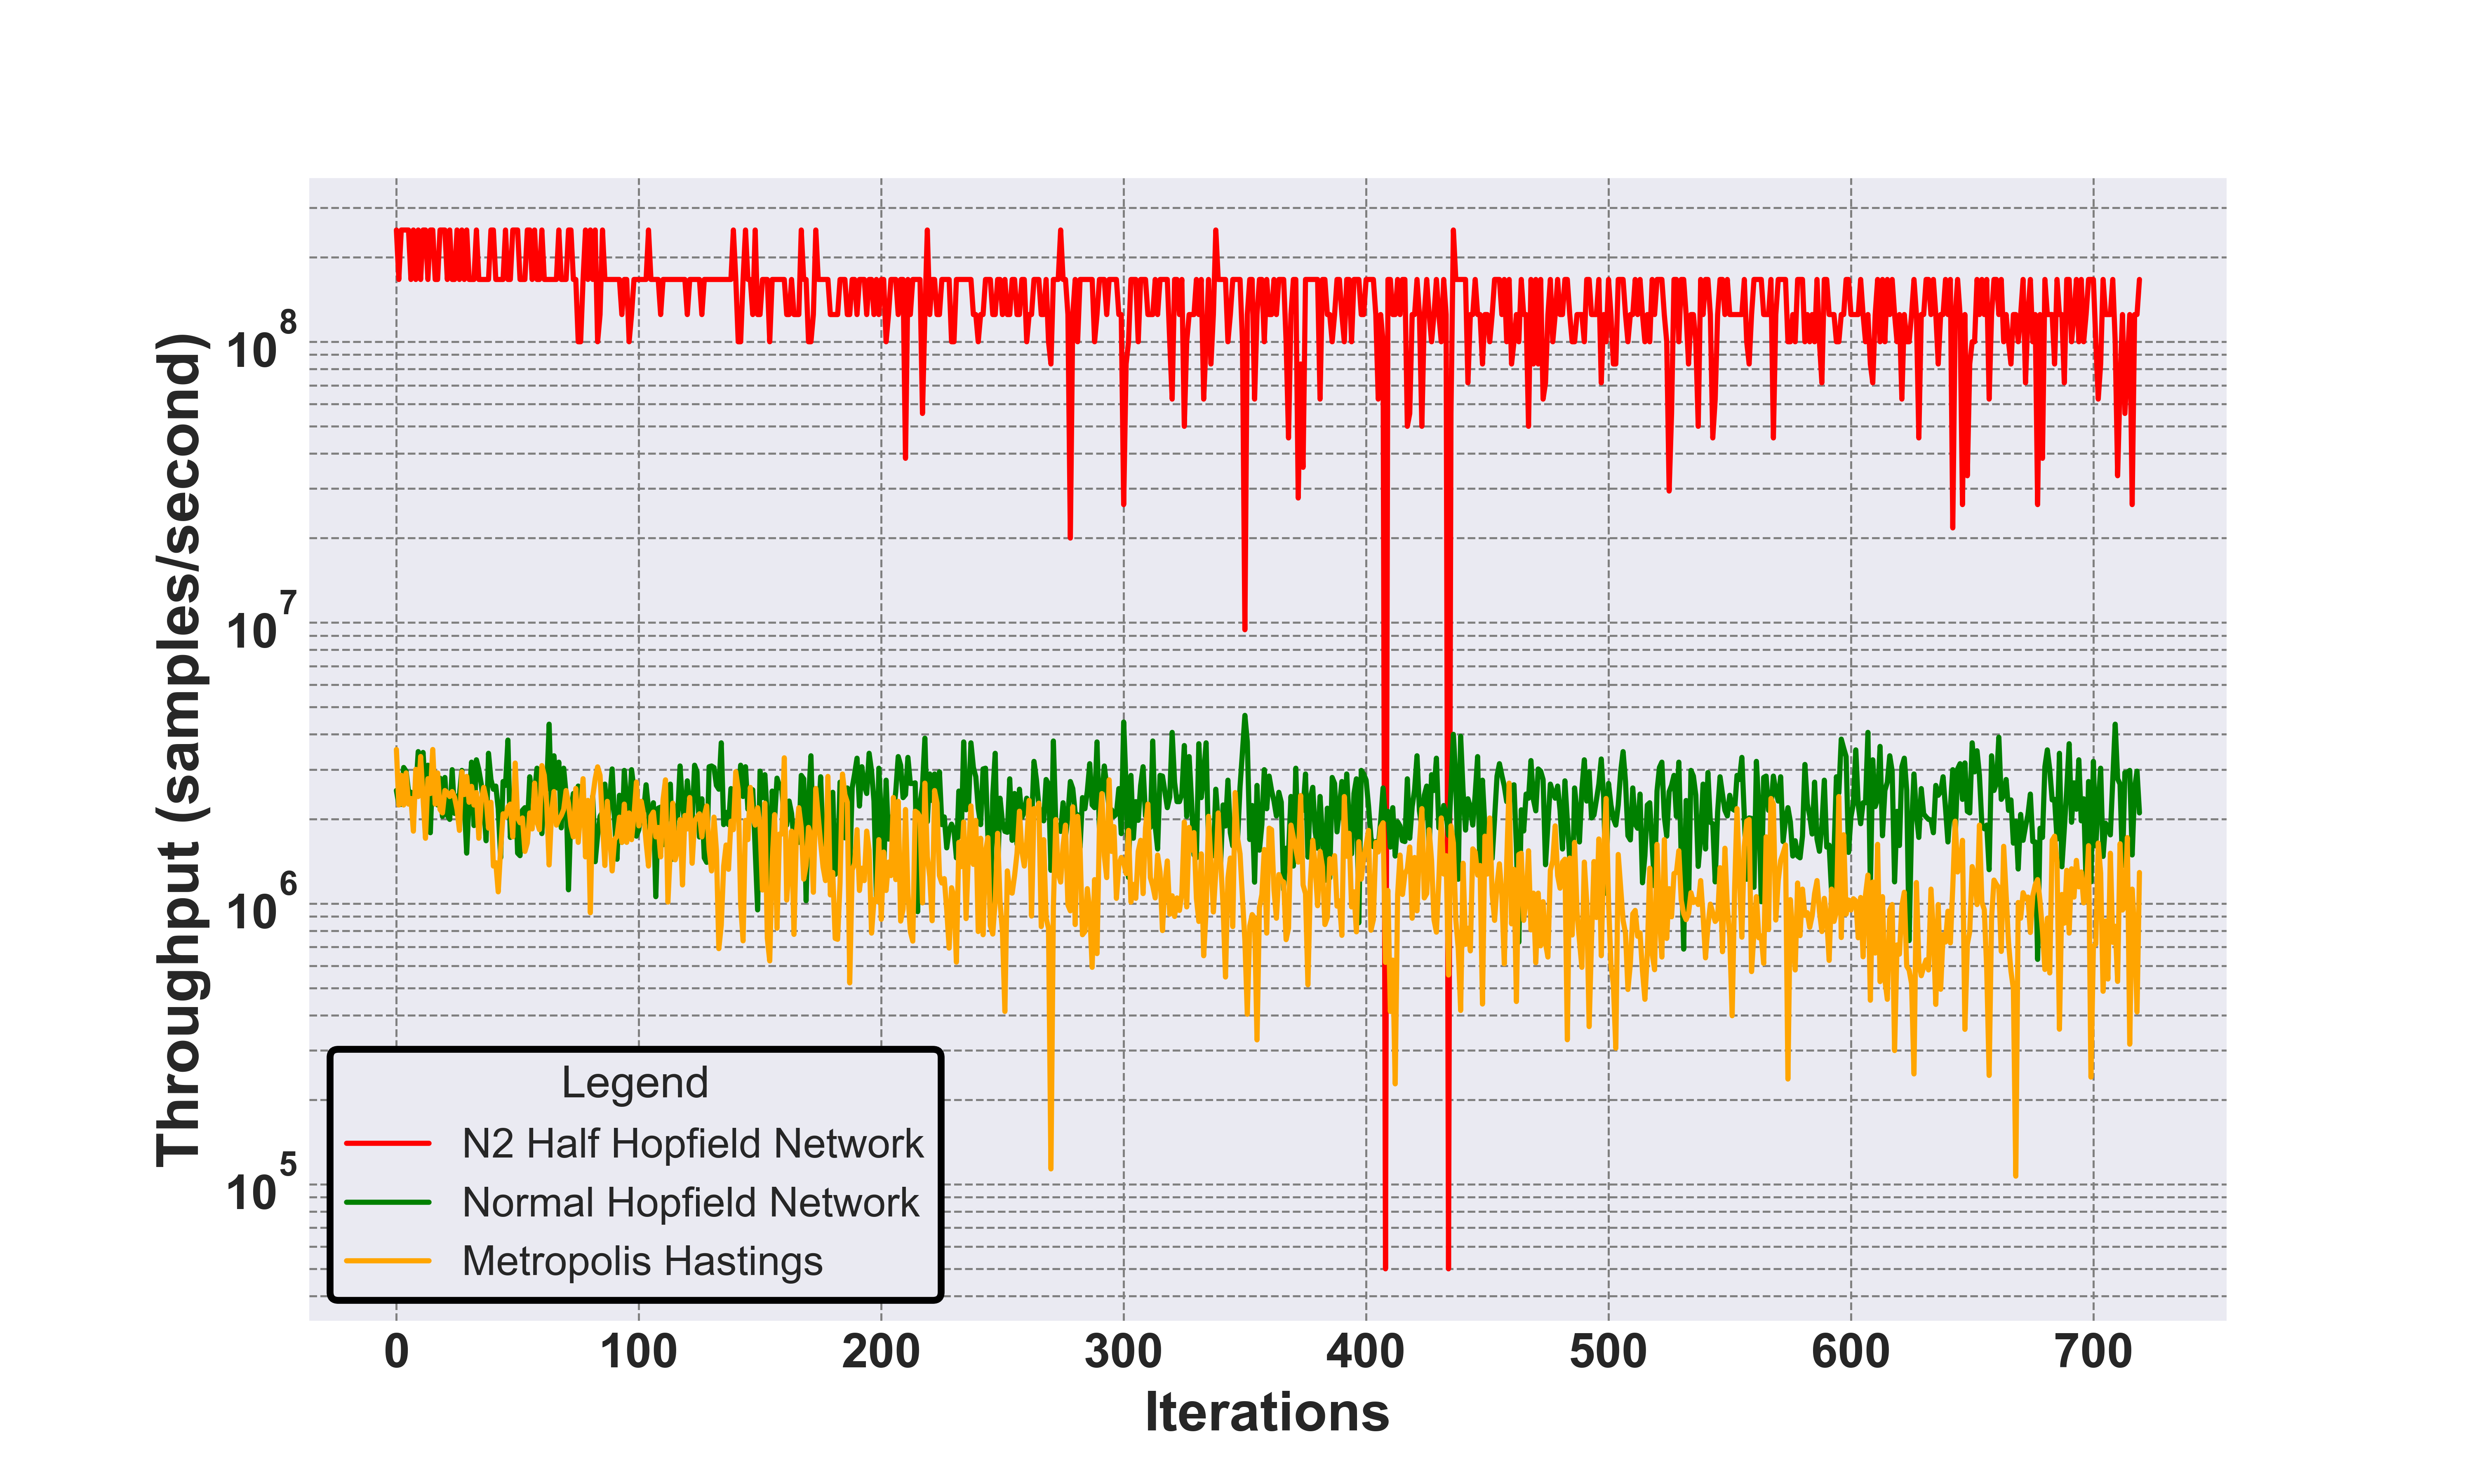
\includegraphics[width=0.8\linewidth]{graphics/Visualisierungen_throughput_MODIFIED.png}
    \caption{Comparison throughput literature}
    \label{Comparison_throughput_literature_3}
\end{figure}
It is visible that the single spin Hopfield Network initially has a equal throughput compared to Metropolis Hastings 
but over time Metropolis Hastings falls off. The average is \textbf{1.37 megasamples per second} compared to to the 2.3
megsamples per second of the single spin Hopfield Network, which therefore is \(\mathbf{1.67x}\) faster.
A second paper to compare the throughput with takes the 144megsamples/second of the N/2 Half approach and compares it
with the estimated sampling rates of analog bandwiths.\footcite[cf.][7]{bohmNoiseinjectedAnalogIsing2022}
Beneficial is that the paper also uses the autocorrelation function with the same threshold for statistically independent samples (1/e).
In a direct comparison for a network size of 164 neurons the performance of the N/2 Half approach beats the 100MHZ analog bandwith slightly.
Nevertheless, the workload differs slightly, necessitating a cautious approach to the comparison.

Lastly, another paper established a comparison of probalistic hardware accelerators. Here, ``time per sweep(ns)'' is used, wich measures the duration required
once all spins have touched like in the other paper.\footcite[cf.][2]{aaditAcceleratingAdaptiveParallel2023}
With the clock cylce of 2ns and 11.2 required iterations (900 neurons in the network) the resulting time per sweep is \(\mathbf{22.4ns}\)
, which is \textbf{slower} than the \ac{FPGA}-based PC (5.83ns) and Google’s
multiple TPU (no exact value). 
Although the time per sweep is competitive and surpasses some probabilistic accelerators it is important to consider that the workloads differ and a direct comparison is not possible.
A visual representation of the probabilistic accelerators can be seen in following figure\ref{Comparison_throughput_literature_2}:
\begin{figure}[H]
    \centering
    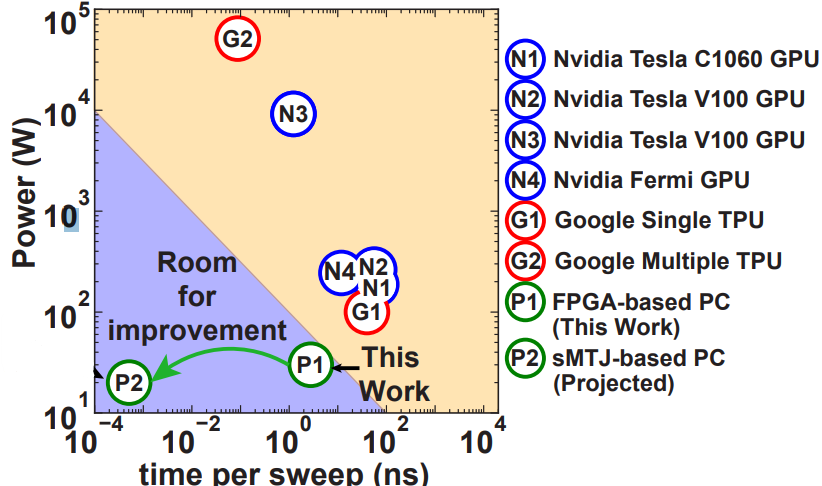
\includegraphics[width=0.55\linewidth]{graphics/Troughput_comparison.png}
    \caption{Comparison throughput with Metropolis Hastings}
    \label{Comparison_throughput_literature_2}
\end{figure}

\section{Energy consumption}

Although the computation speed aligns with other probabilistic accelerators, the energy consumption here clearly sets it apart.
The resulsts show that the average sampling iteration requires beween 50 piko Joules and 20 piko Joules decreasing with ongoing training iterations.
Furthermore, to make these numbers comparable the power requiered is only \(\mathbf{22.5mW}\) decreasing over the training iterations to just under \(\mathbf{10mW}\).
This enables a complete training of the neural network with the consumption of only \(\mathbf{6 mJ}\) (720 Training iterations).
The training is simulated on a CPU\footnote{\texttt{Intel i7-10610U, 1.80GHz, 2304 Mhz, 4 Core(s), 8 Logical Processor(s)}}, which took around 30minutes and has a thermal design power of 15W.
Therefore, the training used \textbf{27.000Joules}, which consumes \(\mathbf{460.000 \ x}\) more energy compared to the \ac{mem-HNN}.
For a complete comparison the energy consumption of the digital computer and the communication to the analog accelerator would need to be meassured 
and int total make the result slightly worse. 
The paper\ref{Comparison_throughput_literature_2} used 7200 neruons in the system for the established comparison. 
Hence, to make it comparable the power consumption of the \ac{mem-HNN}, the power needs to be multiplied by the factor of the neurons \(\mathbf{7200/164=43}\).\footcite[cf.][2]{aaditAcceleratingAdaptiveParallel2023}.
Thus, the new power consumption is \(\mathbf{22.5mW * 43 = 0.9675W}\), which compared to the listed accelerators
where power consumption starts at \(\mathbf{10^1 \, W}\) and can reach nearly \(\mathbf{10^4 \, W}\), is at least \(\mathbf{15 \times}\) worse than the \ac{mem-HNN}.
In total the \ac{mem-HNN} has an competitive computing speed like the \ac{FPGA}s but has an significant advantage when comparing the energy consumption.
Since the aim is to achieve new applications for more sustainable AI models on this \ac{ASIC} accelerator, 
this can be seen as great achievement.

\section{diffusion}
Now that the results have been processed and are comparable, the diffusion phase of the \ac{DSR} framework 
requires that the results are generally made available to the public. 
The results and the implementation are handed over to HP Labs and are used as 
bases for further research.
The goal is to further develop the complete implementation of the model on the physical hardware accelerator.
Furthermore, it is planned to take the results and include them in an upcoming paper that is presented
at TechCon, which is an HPE internal research fair. 
In addition to that, the results are planned to be included and shown at public fairs that HPE plans on going in near future.
Lastly, this bachelor thesis is submitted to the DHBW-Stuttgart for assessment. 


WICHTIG

Therefore, Boltzmann Machines can indeed be efficiently implemented on the physics-inspired Hardware accelerator by analog noise injection. 